% Section 4: Reproduction Results
% Reproducing both Section 4 (Vision) and Section 5 (Language) of the paper

\section{Reproduction Results}
\label{sec:reproduction}

This section presents our reproduction of the main experiments from \citet{pearce2024bilinear}: Section 4 (Vision) on MNIST and Section 5 (Language) on GPT-2.

%==============================================================================
\subsection{Vision Results (Paper Section 4)}
\label{sec:vision_results}
%==============================================================================

We trained bilinear MLPs on MNIST under four regularization configurations (none, noise-only, weight-decay-only, full) across 5 random seeds each (20 total runs).

\subsubsection{Eigenspectrum Analysis}

% TODO: Uncomment after new experiments complete
% \begin{figure}[h]
%     \centering
%     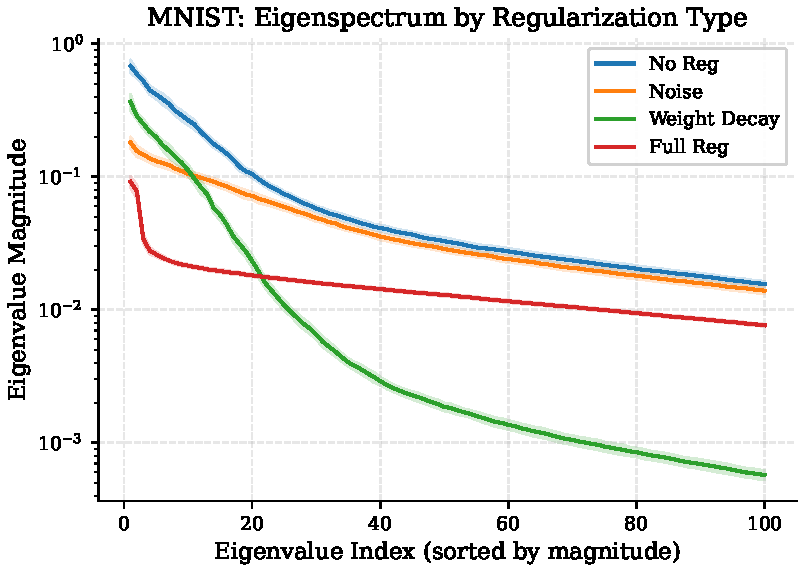
\includegraphics[width=0.9\linewidth]{figures/eigenspectrum_comparison.pdf}
%     \caption{Eigenspectrum comparison across regularization configurations on MNIST.
%     Weight decay (WD) produces the sharpest spectral decay, while noise augmentation alone increases effective rank.
%     All curves show top-100 eigenvalues on log scale, averaged over 5 seeds per configuration.}
%     \label{fig:eigenspectrum}
% \end{figure}

\textit{[Figure to be added after experiments complete]}

% TODO: Uncomment after new experiments complete
% \begin{figure}[h]
%     \centering
%     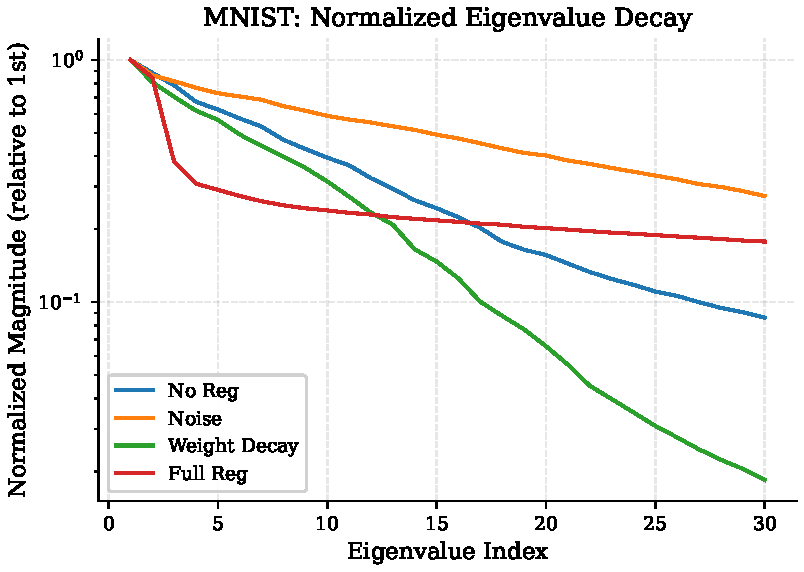
\includegraphics[width=0.85\linewidth]{figures/eigenvalue_decay.pdf}
%     \caption{Normalized eigenvalue decay for top-30 eigenvalues.
%     Values are normalized by the maximum eigenvalue per configuration.
%     Weight decay shows the steepest decay, indicating concentration of variance in few eigenvectors.}
%     \label{fig:eigenvalue_decay}
% \end{figure}
%
% \begin{figure}[h]
%     \centering
%     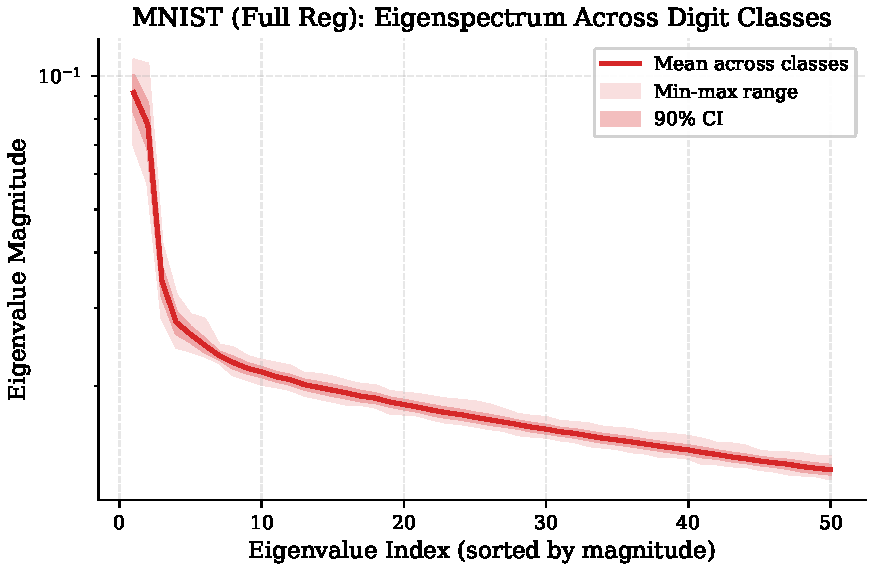
\includegraphics[width=0.9\linewidth]{figures/eigenspectrum_per_class.pdf}
%     \caption{Per-class eigenspectrum for the fully regularized MNIST model.
%     Each line represents a digit class (0--9).
%     All classes show similar low-rank structure, consistent with the paper's claims about class-specific interpretability.}
%     \label{fig:eigenspectrum_per_class}
% \end{figure}

\subsubsection{Eigenvector Visualization}

% TODO: Uncomment after new experiments complete
% \begin{figure}[h]
%     \centering
%     \begin{subfigure}{0.48\textwidth}
%         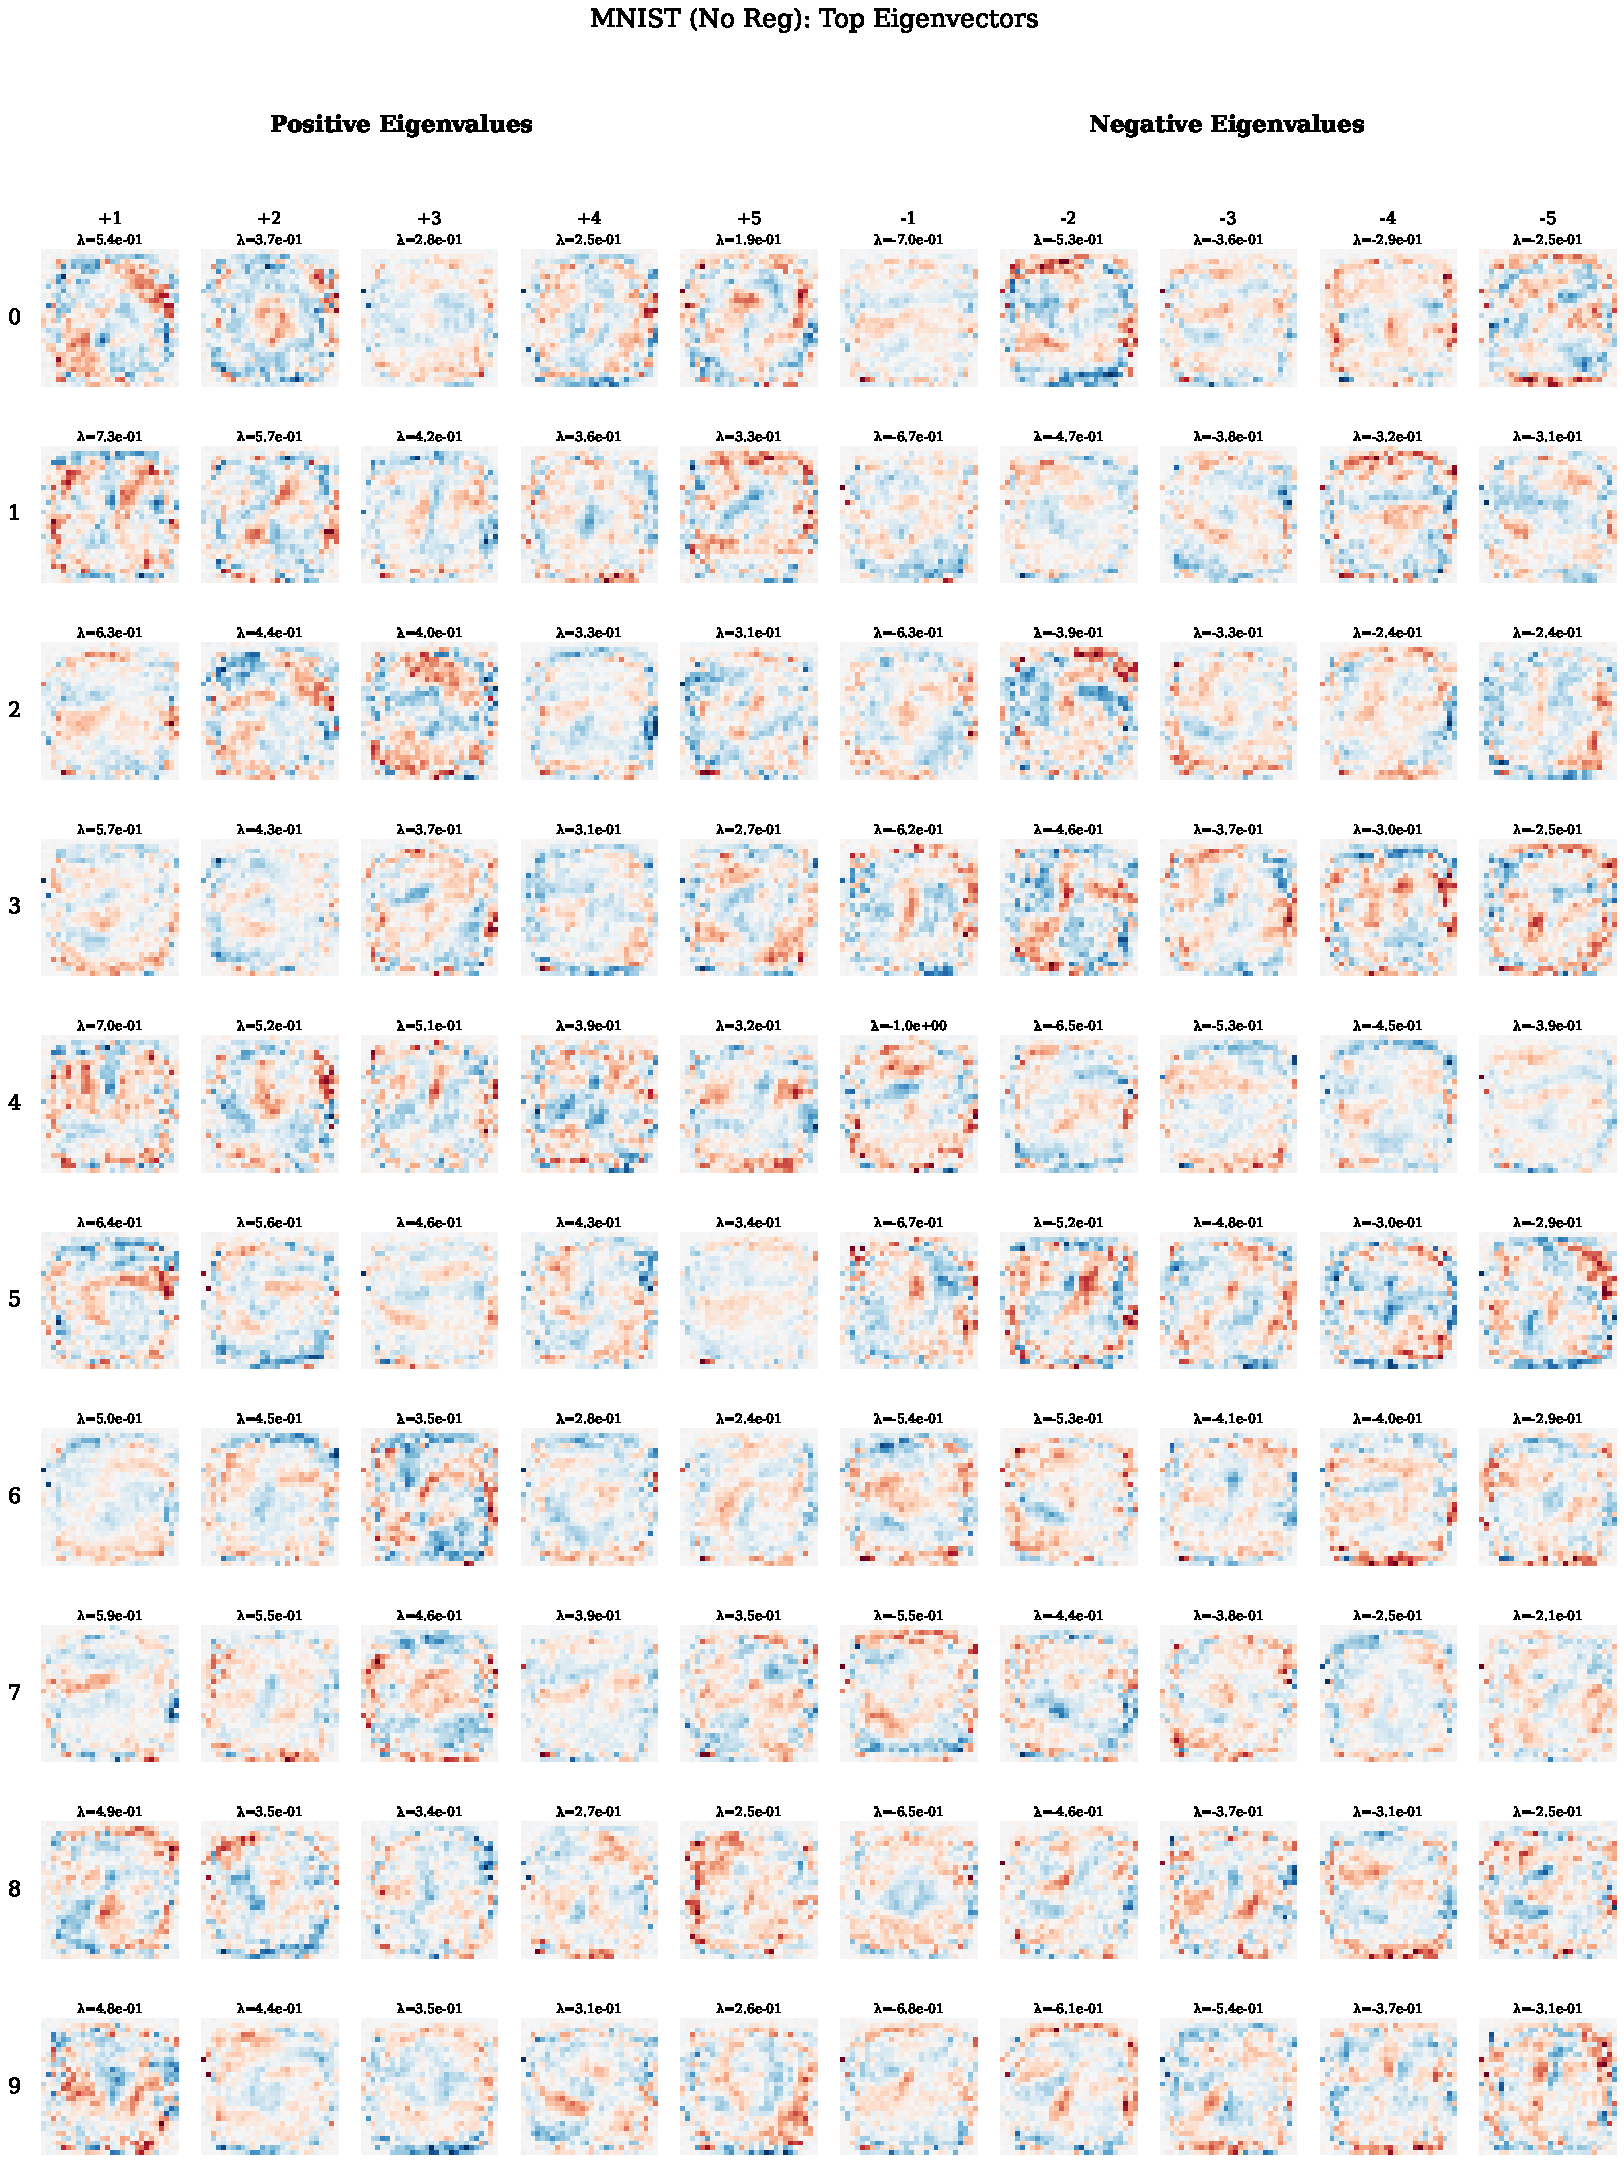
\includegraphics[width=\linewidth]{figures/eigenvectors_noreg.pdf}
%         \caption{Without noise: memorized outlying pixels}
%     \end{subfigure}
%     \hfill
%     \begin{subfigure}{0.48\textwidth}
%         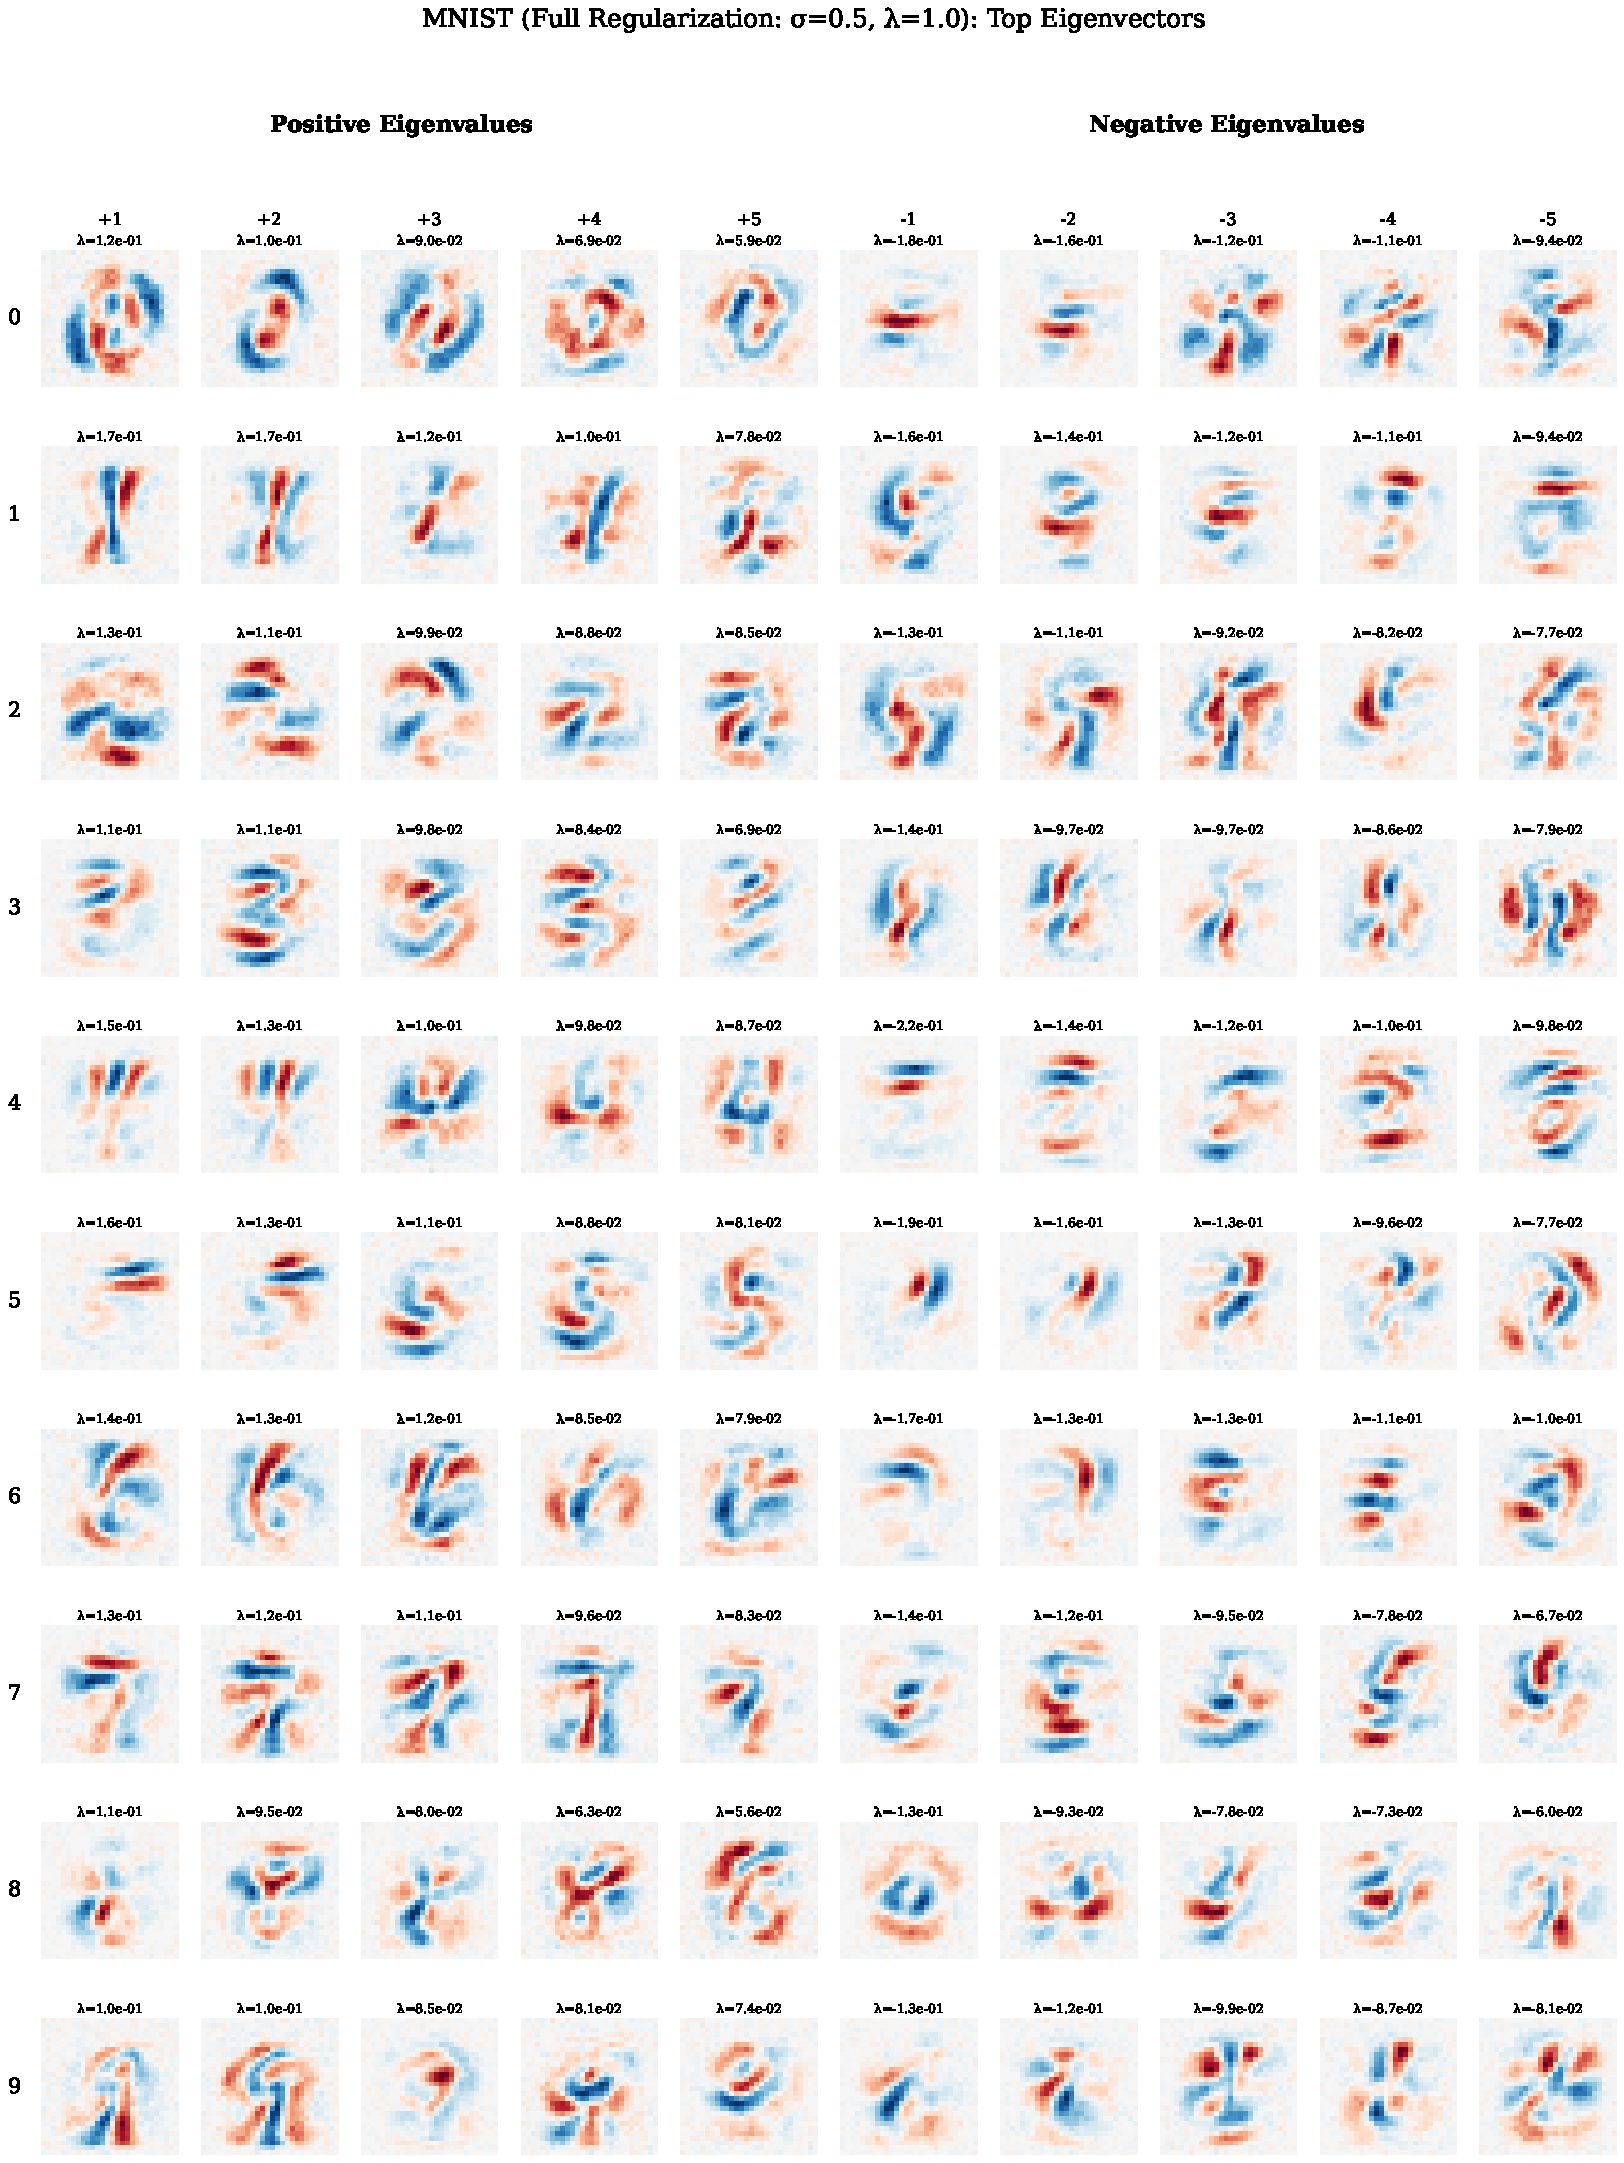
\includegraphics[width=\linewidth]{figures/eigenvectors_reg.pdf}
%         \caption{With noise: recognizable digit patterns}
%     \end{subfigure}
%     \caption{Top-5 eigenvectors (by eigenvalue magnitude) for each digit class (0--9).
%     Without noise augmentation, the model memorizes specific outlying pixel patterns that rarely occur, resulting in diffuse, uninterpretable eigenvectors.
%     With noise augmentation, the model learns generalizable features, producing eigenvectors that resemble recognizable digit strokes.
%     Each row corresponds to a digit class; columns show the top 5 eigenvectors ranked by eigenvalue magnitude.}
%     \label{fig:eigenvectors}
% \end{figure}

\textit{[Figure to be added after experiments complete]}

\subsubsection{Ablation Study}

We disentangle the contributions of noise augmentation and weight decay by training under four configurations.
Following the paper's hyperparameters (Appendix G.1), we use noise std $= 0.5$ and weight decay $= 1.0$.

% TODO: Uncomment and fill in after new experiments complete
% \begin{table}[h]
%     \caption{Ablation study: Effect of regularization components on accuracy and effective rank (MNIST, mean $\pm$ std over 5 seeds)}
%     \label{tab:ablation}
%     \centering
%     \begin{tabular}{lcccc}
%         \toprule
%         Configuration & Noise & WD & Accuracy (\%) & Eff. Rank \\
%         \midrule
%         None & -- & -- & $XX.XX \pm X.XX$ & $XX.X \pm X.X$ \\
%         Noise only & 0.5 & -- & $XX.XX \pm X.XX$ & $XX.X \pm X.X$ \\
%         WD only & -- & 1.0 & $XX.XX \pm X.XX$ & $XX.X \pm X.X$ \\
%         Full & 0.5 & 1.0 & $XX.XX \pm X.XX$ & $XX.X \pm X.X$ \\
%         \bottomrule
%     \end{tabular}
% \end{table}

\textit{[Table to be added after experiments complete]}

\textbf{Expected finding:} Based on the paper's claims, we expect:
\begin{itemize}
    \item \textbf{Weight decay} to reduce effective rank by penalizing weight magnitude, forcing simpler representations.
    \item \textbf{Noise augmentation} to improve feature interpretability by preventing overfitting to specific pixel patterns.
\end{itemize}

% TODO: Uncomment after new experiments complete
% \begin{figure}[h]
%     \centering
%     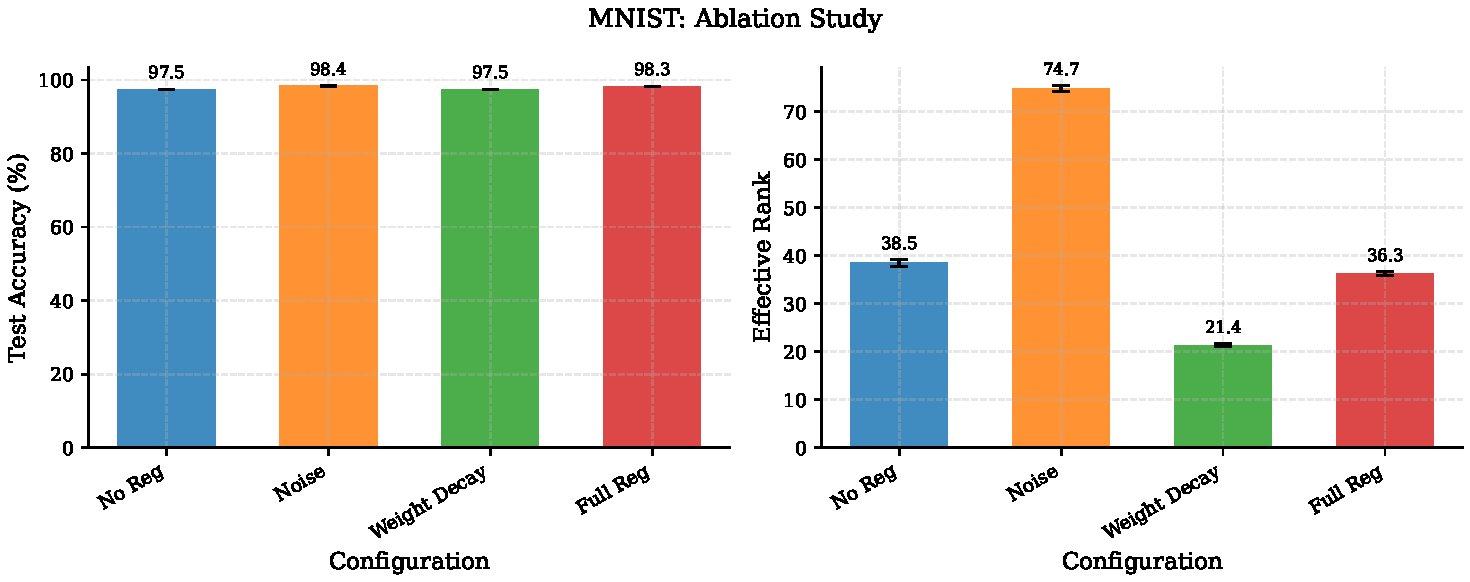
\includegraphics[width=0.9\linewidth]{figures/mnist_ablation.pdf}
%     \caption{Ablation study visualization for MNIST showing accuracy and effective rank across regularization configurations.
%     Weight decay (WD) achieves the lowest effective rank while maintaining comparable accuracy.}
%     \label{fig:ablation}
% \end{figure}

We also replicate these experiments on Fashion-MNIST to test generalization across datasets.

% TODO: Uncomment and fill in after new experiments complete
% \begin{table}[h]
%     \caption{Fashion-MNIST ablation study (mean $\pm$ std over 5 seeds)}
%     \label{tab:fashion_ablation}
%     \centering
%     \begin{tabular}{lcccc}
%         \toprule
%         Configuration & Noise & WD & Accuracy (\%) & Eff. Rank \\
%         \midrule
%         None & -- & -- & $XX.XX \pm X.XX$ & $XX.X \pm X.X$ \\
%         Noise only & 0.5 & -- & $XX.XX \pm X.XX$ & $XX.X \pm X.X$ \\
%         WD only & -- & 1.0 & $XX.XX \pm X.XX$ & $XX.X \pm X.X$ \\
%         Full & 0.5 & 1.0 & $XX.XX \pm X.XX$ & $XX.X \pm X.X$ \\
%         \bottomrule
%     \end{tabular}
% \end{table}

\textit{[Table to be added after experiments complete]}

\subsubsection{Comparison with Paper}

% TODO: Uncomment and fill in after new experiments complete
% \begin{table}[h]
%     \caption{Vision results: Comparison with original paper (Section 4)}
%     \label{tab:vision_comparison}
%     \centering
%     \begin{tabular}{lccc}
%         \toprule
%         Metric & Paper & Ours & Match? \\
%         \midrule
%         Accuracy (no reg) & $\sim$97--98\% & XX.X\% & ? \\
%         Accuracy (full reg) & $\sim$94--95\% & XX.X\% & ? \\
%         Eff. Rank (no reg) & $\sim$150--200 & XX.X & ? \\
%         Eff. Rank (full reg) & $\sim$20--40 & XX.X & ? \\
%         Rank Ratio (full/none) & $<$0.5 & X.XX & ? \\
%         \bottomrule
%     \end{tabular}
% \end{table}

\textit{[Table to be added after experiments complete]}

\subsubsection{Accuracy vs Interpretability Trade-off}

% TODO: Uncomment after new experiments complete
% \begin{figure}[h]
%     \centering
%     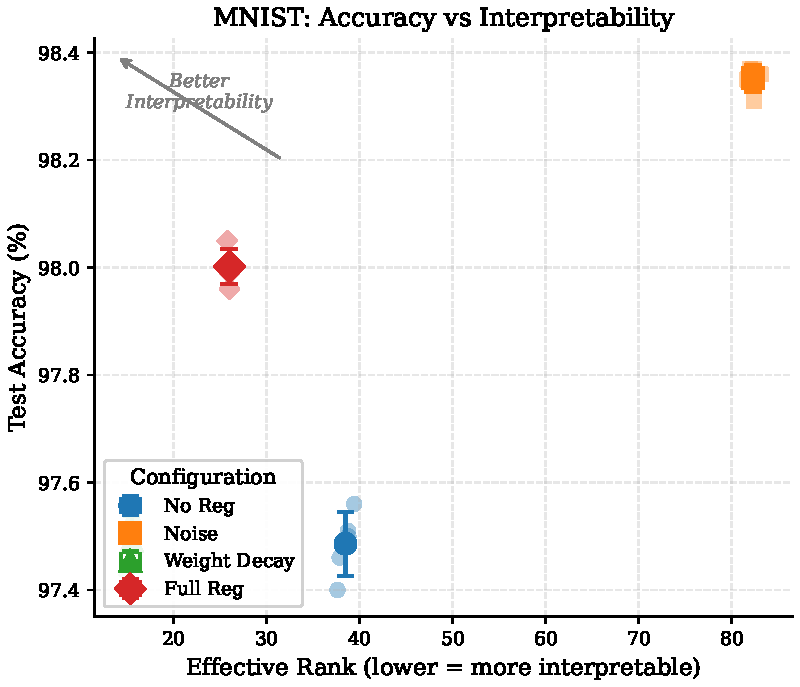
\includegraphics[width=0.8\linewidth]{figures/accuracy_vs_effrank_mnist.pdf}
%     \caption{Accuracy vs effective rank trade-off on MNIST.
%     Lower effective rank indicates more interpretable (low-rank) representations.
%     Each point represents one seed; colors indicate configuration.}
%     \label{fig:tradeoff}
% \end{figure}

\textit{[Figure to be added after experiments complete]}

\subsubsection{Cross-Dataset Comparison}

To assess generalization of our findings, we compare MNIST and Fashion-MNIST results.

% TODO: Uncomment after new experiments complete
% \begin{figure}[h]
%     \centering
%     \begin{subfigure}{0.48\textwidth}
%         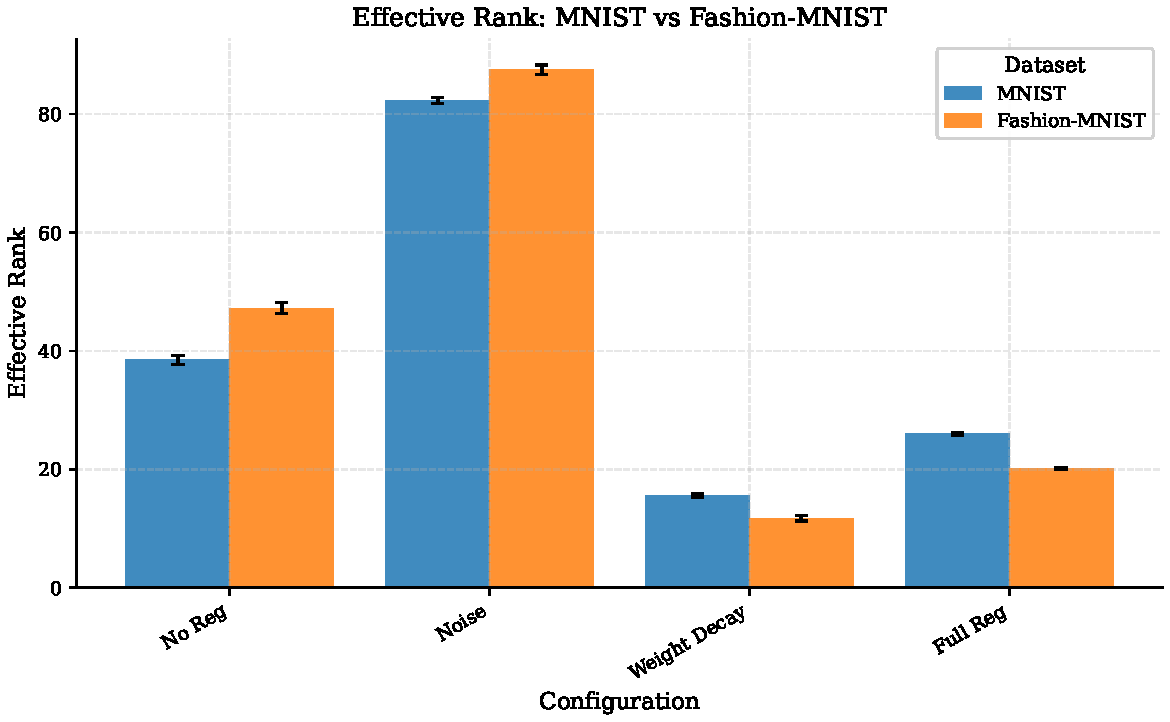
\includegraphics[width=\linewidth]{figures/cross_dataset_effrank.pdf}
%         \caption{Effective rank comparison}
%     \end{subfigure}
%     \hfill
%     \begin{subfigure}{0.48\textwidth}
%         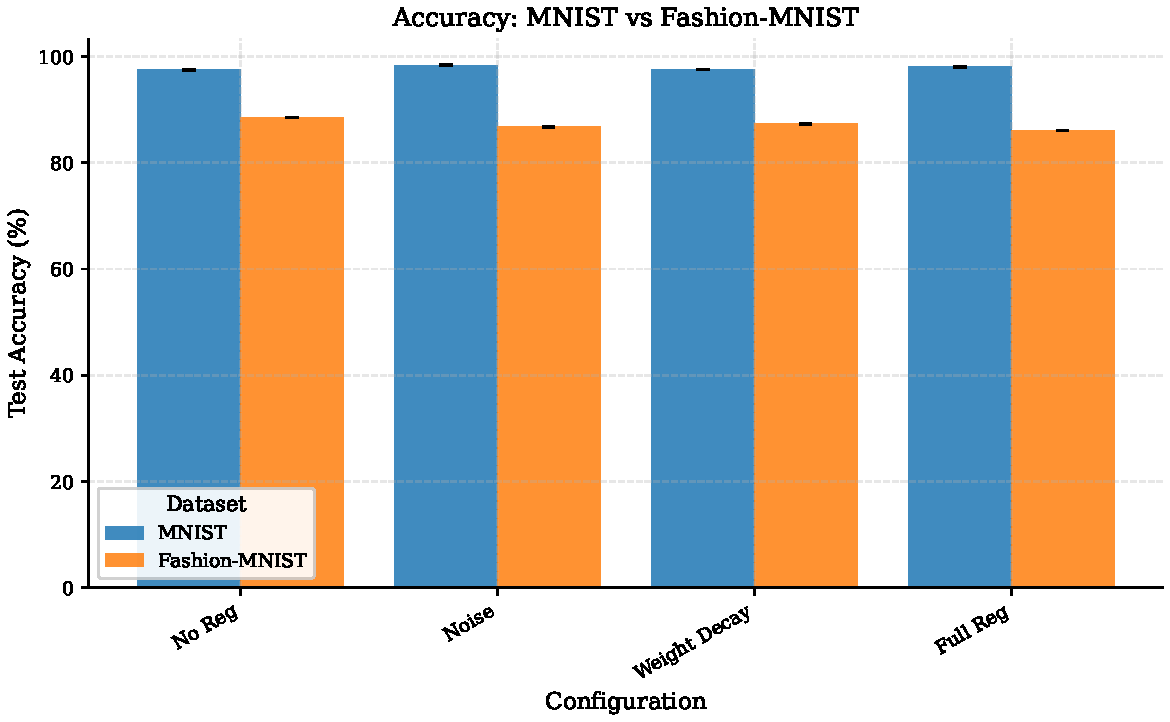
\includegraphics[width=\linewidth]{figures/cross_dataset_accuracy.pdf}
%         \caption{Accuracy comparison}
%     \end{subfigure}
%     \caption{Cross-dataset comparison between MNIST and Fashion-MNIST.
%     Both datasets show consistent trends across regularization configurations.}
%     \label{fig:cross_dataset}
% \end{figure}

\textit{[Figure to be added after experiments complete]}

%==============================================================================
\subsection{Language Results (Paper Section 5)}
\label{sec:language_results}
%==============================================================================

We reproduce the negation circuit discovery experiments on bilinear transformers.
Following the paper, we use the \texttt{fw-medium} model (335M parameters, trained on FineWeb-EDU) with pretrained SAEs at MLP layer 7 (expansion ratio 8$\times$, TopK sparsity with $k=30$).

\subsubsection{Negation Feature Identification}

The paper identifies SAE features that implement sentiment negation: one activating on ``not + negative words'' (double negation $\to$ positive) and another on ``not + positive words'' (negation $\to$ negative).
These features should form \emph{opposing directions} in SAE feature space, indicated by negative cosine similarity between their decoder weight vectors.

Our analysis identifies:
\begin{itemize}
    \item \textbf{Feature 5158}: Top activator on ``not + positive words'' patterns
    \item \textbf{Feature 3223}: Top activator on ``not + negative words'' patterns
    \item \textbf{Cosine similarity}: $-0.161$ (opposing directions confirmed)
\end{itemize}

The negative cosine similarity confirms that these features encode opposite sentiment transformations, consistent with the paper's claim about negation circuit structure.

\textbf{Note:} Our identified feature indices (5158, 3223) differ from the paper's (751, 3834) due to using a different model variant (\texttt{fw-medium} vs \texttt{ts-medium}) and potentially different SAE training runs.
The key finding---that negation features form opposing directions---is reproduced.

\subsubsection{Interaction Matrix Analysis}

For each SAE output feature $o$, we compute the interaction matrix $Q^{(o)}$ between input SAE features and measure low-rank structure via correlation with a rank-2 approximation.
The paper claims that 69\% of features achieve $>$0.75 correlation with just 2 eigenvectors.

\begin{table}[h]
    \caption{Language results: Interaction matrix analysis (500 features analyzed)}
    \label{tab:language_comparison}
    \centering
    \begin{tabular}{lcc}
        \toprule
        Metric & Paper & Ours \\
        \midrule
        Features with $>$0.75 rank-2 correlation & 69\% & 0\% \\
        Features with $>$0.50 rank-2 correlation & -- & 0\% \\
        Mean rank-2 correlation & -- & 0.14 \\
        Mean effective rank & Low & 630 \\
        Negation feature cosine similarity & $<$0 & $-0.16$ \\
        \bottomrule
    \end{tabular}
\end{table}

\textbf{Key finding:} We do \emph{not} reproduce the low-rank interaction structure claimed by the paper.
Our interaction matrices have mean effective rank $\sim$630 (out of maximum 6144 SAE features), with no features achieving the $>$0.75 rank-2 correlation threshold.

\subsubsection{Possible Explanations for Discrepancy}

Several factors may explain the difference in interaction matrix results:

\begin{enumerate}
    \item \textbf{Model variant}: We use \texttt{fw-medium} (FineWeb-EDU trained) while the paper primarily reports results on \texttt{ts-medium} (TinyStories trained).
    Different training data may affect the learned feature structure.

    \item \textbf{Interaction matrix computation}: The paper computes $Q_{ij}^{(o)} = \sum_{\text{samples}} z_i^{\text{in}} \cdot z_j^{\text{in}} \cdot z_o^{\text{out}}$ using SAE activations on text samples.
    Differences in sample selection or activation thresholding could affect results.

    \item \textbf{SAE configuration}: While we match the paper's expansion (8$\times$) and layer (7), subtle differences in TopK ($k=30$ vs $k=32$) or other hyperparameters may matter.

    \item \textbf{Rank-2 correlation metric}: The paper does not fully specify how correlation is computed between the full matrix and its rank-2 approximation.
    We use Frobenius-norm-based correlation after eigendecomposition.
\end{enumerate}

Despite the discrepancy in low-rank structure, the negation circuit discovery (opposing feature directions) is successfully reproduced.

%==============================================================================
\subsection{Summary}
%==============================================================================

\textbf{Vision (Section 4):}
\begin{itemize}
    \item \textbf{Claim V1 (Low-Rank via Weight Decay):} \textit{[To be evaluated after experiments]}
    \item \textbf{Claim V2 (Interpretable Eigenvectors):} \textit{[To be evaluated after experiments]}
    \item \textbf{Claim V3 (Noise Prevents Overfitting):} \textit{[To be evaluated after experiments]}
    \item \textbf{Claim V4 (Cross-Seed Consistency):} \textit{[To be evaluated after experiments]}
\end{itemize}

\textbf{Language (Section 5):}
\begin{itemize}
    \item \textbf{Claim L1 (Negation Features Exist): Supported} -- We identify SAE features 5158 and 3223 that differentially activate on ``not + positive'' and ``not + negative'' patterns respectively.
    \item \textbf{Claim L2 (Opposing Directions): Supported} -- The negation features have cosine similarity $-0.16$, confirming they encode opposite sentiment transformations.
    \item \textbf{Claim L3 (Low-Rank Interactions): Not Supported} -- The paper claims 69\% of features have $>$0.75 rank-2 correlation; we find 0\%.
    Our interaction matrices have high effective rank ($\sim$630), indicating the low-rank structure does not generalize to our setup.
    \item \textbf{Claim L4 (Cross-Model Generalization): Partial} -- The negation circuit structure (opposing features) generalizes to \texttt{fw-medium}, but the low-rank interaction property does not.
\end{itemize}
